\documentclass[letterpaper, 10pt]{article}

%---- packages----------------------------%
\usepackage{titling}
\usepackage{hyperref}
\usepackage{ulem}
\usepackage{booktabs}
\usepackage{siunitx}
\usepackage{graphicx} % documentation: http://ftp.math.purdue.edu/mirrors/ctan.org/macros/latex/required/graphics/grfguide.pdf
\usepackage{amsmath}
\usepackage{siunitx}
\usepackage{natbib}
%----------------------------------------------%

\begin{document}

\setlength{\droptitle}{-10em} 
\title{\large\textbf{Parameterization of DEMENTpy across the Southern California Climate Gradient}\vspace{0em}}
\author{\normalsize\textbf{Bin Wang\textsuperscript{1}, Steven D. Allison\textsuperscript{1,2}}\vspace{1em} \\
\textsuperscript{1}Ecology and Evolutionary Biology, \textsuperscript{2}Earth System Science \\
University of California Irvine\vspace{-0em} \\
Email: bwang7@uci.edu} 
\date{\normalsize August, 2020\vspace{0em}}
\maketitle


This document serves to detail how the DEMENTpy inputs were prepared for each of the five sites simulated across the climate gradient (\textbf{Figure 1}). In combination with the Jupyter Notebooks(.ipynb) provided, readers or those who are interested are supposed to be able to reproduce the preparation.

In detail, inputs including water potential, soil temperature, and litter chemistry were processed and derived. Water potential was derived from precipitation via an intermediate step of converting the precipitation data. Code underlying all this processing is accessible at a GitHub Repo (\url{https://github.com/bioatmosphere/microbiome-climate-gradient.git}).

% figure of the location of the five sites
\begin{figure}[h]
\centering
  %\begin{center}
      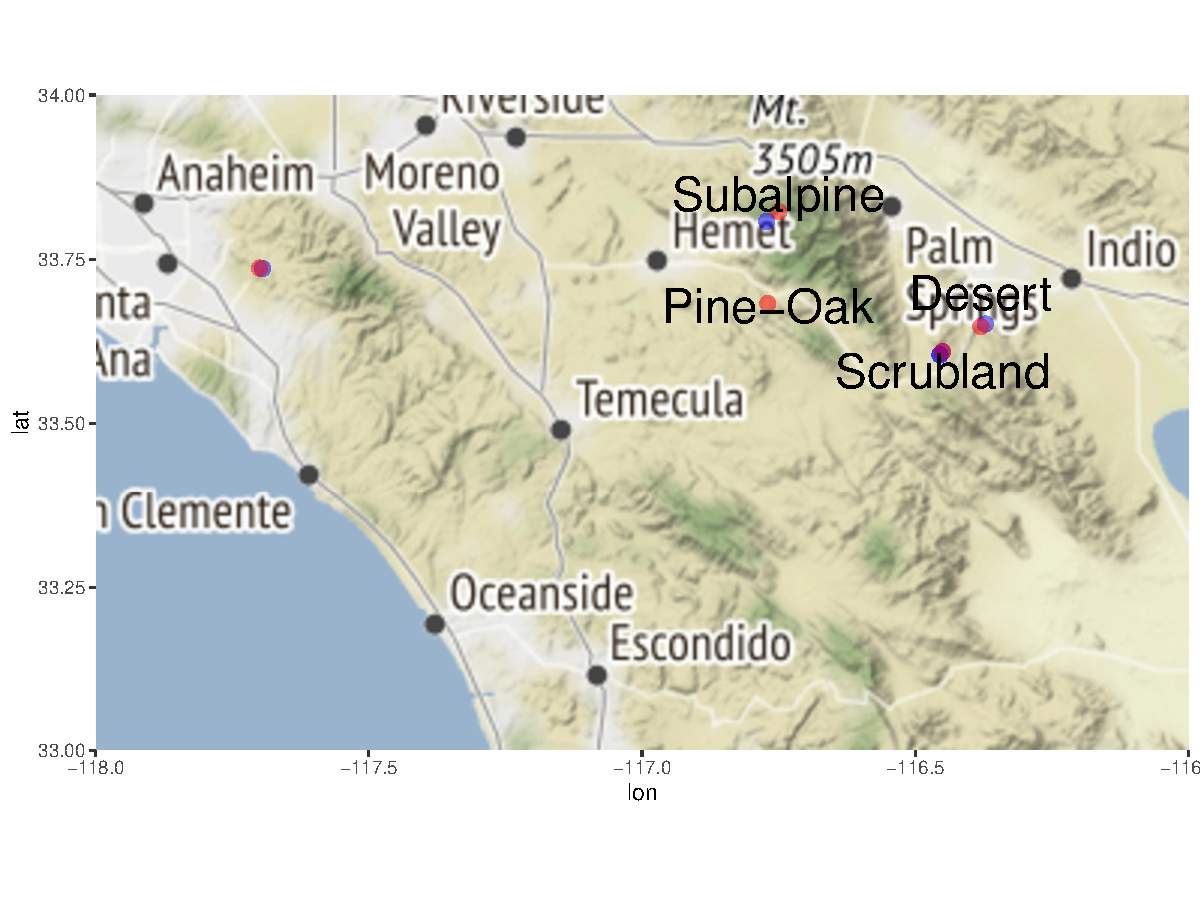
\includegraphics[scale=0.5]{site_location_v1.pdf}
      \caption{Location of the five sites.}
      \label{fig: figure 1}
  %\end{center}
\end{figure}

\section{\large Ecosystems across the Southern California climate gradient}

% table of the basic features of the five sites 
\begin{table}[h!]
  \begin{center}
    \caption{Five sites across the climate gradient.}
    \label{tab: table1}
    \begin{tabular}{lccc}
      \toprule % <-- Toprule here
      \textbf{Site} & \textbf{Latitude} & \textbf{Longitude} & \textbf{Elevation}\\
      %$\alpha$ & $\beta$ & $\gamma$ \\
      \midrule % <-- Midrule here
      Desert       & 33.648 & -116.38 & 275\\
      Scrubland & 33.610 & -116.45 & 1280\\
      Grassland & 33.737 & -117.70 & 470\\
      Pine-Oak  & 33.683 & -116.77  & 1710\\
      Subalpine & 33.823 & -116.75  & 2250\\
      \bottomrule % <-- Bottomrule here
    \end{tabular}
  \end{center}
\end{table}

All five sites (\textbf{Table 1}) are located on granitic parent material and experience Mediterranean precipitation patterns (cool, wet winters; hot, dry summers). This climate gradient covers a temperature range from ... to...



\section{\large Climate Forcing}

\subsection{Precipitation}
Longterm daily precipitation data were accessed from various sources for the five sites:

\textbf{Desert}: daily precipitation data from Boyd Deep Canyon California accessible at \url{https://wrcc.dri.edu/cgi-bin/rawMAIN.pl?caucde}

\textbf{Scrubland}: daily precipitation data from Burns Pinon Ridge Reserve California accessible at \url{https://wrcc.dri.edu/cgi-bin/rawMAIN.pl?caucbu}

\textbf{Grassland}:

\textbf{Pine-Oak}: daily precipitation data from James Reserve Station, California available at \url{https://wrcc.dri.edu/cgi-bin/rawMAIN.pl?caucja}

\textbf{Subalpine}: Since there was no station directly next to the Subalpine site, the precipitation at this site is likely underestimated. In Glassman et al. (2019), precipitation was averaged from three NOAA weather stations with heated gauges accounting for snow (USC00045091; US1CARV0002; and USC00044211): \url{https://www.ncdc.noaa.gov/cdo-web/datasets#GHCND}. Instead, daily precipitation data from station Mt. San Jacinto California (\url{https://raws.dri.edu/cgi-bin/rawMAIN.pl?caCMSJ}) was accessed.


\subsection{Water Potential ($\psi$)}
As there are no direct measurements of water potential ($\theta$; unit: MPa) at different sites across the gradient, an approximate method was applied. This approximation is based on the only available water potential data at the grassland site. With available measurements of water content ($\theta$; unit: g H\textsubscript{2}O g\textsuperscript{-1} wood), daily water potential was derived by Allison and Goulden (2017) at the grassland site for a record of $?????$. This derivation of water potential followed a conversion from water content to water potential as per the equation [Dix 1985, referenced in Allison and Goulden (2017)]:

\begin{equation}
  \psi_{grassland} = -10^{0.118-0.114\log_{10} \theta}
\end{equation}

Water potential of all the other four sites ($\psi_{site}$) were derived by linearly scaling grassland site water potential ($\psi_{grassland}$) based on the Total Annual Precipitation(\textbf{TAP}) across the five sites following:

\begin{equation}
  \psi_{site} = \frac{TAP_{site}}{TAP_{grassland}} \psi_{grassland}
\end{equation}

One reason that make this approximate scaling legitimate is the same Mediterranean precipitation patterns (cool, wet winters; hot, dry summers) of the climate gradient.

\subsection{Temperature (\SI{}{\celsius})}
Soil temperature data at a daily time step was used. These data were available at \url{https://github.com/stevenallison/UCIClimateExperiment/tree/master/updatednames}. 


\section{\large Litter Chemistry and Input}

Litter composition followed field measurements of chemistry at each site as presented in \citep{baker2017extracellular}. As per the observation by Baker and Allison (2017), standing litter pools are largest in the grassland and pine-oak site, reduced in the subalpine site, significantly reduced in the scrubland site, and negligible in the desert site.

\textbf{Phospholipids} are a key component of all cell membranes(\url{https://en.wikipedia.org/wiki/Phospholipid}). In theory, it corresponds to OrgP1 in the model.


%\newpage
\bibliographystyle{authordate1}
\bibliography{references}

\end{document}